\documentclass[prd,preprintnumbers,floatfix,
nofootinbib,superscriptaddress]{revtex4}

%------------------

\usepackage{float}
\usepackage{nicefrac}
\usepackage{mathtools}
\usepackage{amsfonts}
\usepackage{amssymb}
\usepackage{amsmath}
\usepackage{graphicx}
\usepackage{subfigure}
\usepackage{array}
\usepackage{dcolumn}
\usepackage{bm}
\usepackage{esint}
\usepackage{xcolor}
\usepackage{longtable} % long tables
\usepackage{hyperref}
\usepackage{verbatim}
\usepackage{epsfig}
\usepackage{slashed}
\usepackage{color}

\begin{document}
\title{Determination of the spin of $X\to J/\psi\,J/\psi$}

%%%%%%%%%%
\author{Mikhail Mikhasenko}
\email[e-mail: ]{mikhail.mikhasenko@cern.ch}
\affiliation{CERN-EP, CH-1211, Geneva, Switzerland}
%%%%%%%%%%

%%%%%%%%%%
\date{\today}
%%%%%%%%%%

%%%%%%%%%%
\begin{abstract}
The document presents exploratory studies of $J/\psi (\mu^+\mu^-)\,J/\psi (\mu^+\mu^-)$ system.
\end{abstract}
%%%%%%%%%%

\nopagebreak
\maketitle

\definecolor{cola}{rgb}{0.9,0.62,0.0}
\definecolor{colb}{rgb}{0.337, 0.706, 0.914 }
\definecolor{colc}{rgb}{0.0, 0.62, 0.451}

\section{Introduction}

\begin{align*}
  1^-\otimes 1^-: && S:\qquad & {\color{cola} 0^+}\quad {\color{colb} 1^+}\quad {\color{colc} 2^+},\\
                  && P:\qquad & \color{gray} 1^-\quad (0^-,1^-,2^-)\quad (1^-,2^-,3^-),\\
                  && D:\qquad & {\color{colc} 2^+}\quad ({\color{colb} 1^+},{\color{colc} 2^+},3^+)\quad ({\color{cola} 0^+},{\color{colb} 1^+},{\color{colc} 2^+},3^+,4^+),\\
                  && F:\qquad & \color{gray} 3^-\quad (2^-,3^-,4^-)\quad (0^-,1^-,2^-,3^-,4^-),\\
                  && H:\qquad & 4^+\quad (3^+,4^+,5^+)\quad ({\color{colc} 2^+},3^+,4^+,5^+,6^+).
\end{align*}

\begin{align}
    I(\cos\theta_1,\phi_1,\cos\theta_2,\phi_2) &=
    \sum_{\lambda_1,\lambda_2}\sum_{\lambda_1',\lambda_2'}
    \delta_{\lambda_1-\lambda_2,\lambda_1'-\lambda_2'}
    H_{\lambda_1\lambda_2} H_{\lambda_1'\lambda_2'}^{*}
    e^{i(\lambda_1'-\lambda_1)\phi_1}
    e^{i(\lambda_2'-\lambda_2)\phi_2}
    \\ \nonumber
    &\qquad\times
    \sum_{\xi_1}^{\{-1,1\}}
    d_{\lambda_1,\xi_1}^{1}(\theta_1) d_{\lambda_1',\xi_1}^{1}(\theta_1)
    \sum_{\xi_2}^{\{-1,1\}}
    d_{\lambda_2,\xi_2}^{1}(\theta_2) d_{\lambda_2',\xi_2}^{1}(\theta_2).
\end{align}


\section{Angular amplitude}
\begin{align}
  H_{\lambda_1,\lambda_2} = (-1)^{j_1-\lambda_1} \sum_{ls} \sqrt{\frac{2l+1}{2j+1}}
  \left\langle 1,\lambda_1;1,\lambda_2|s,\lambda_1-\lambda_2 \right\rangle
  \left\langle L,0;s,\lambda_1-\lambda_2|j,\lambda_1-\lambda_2 \right\rangle H_{ls}.
\end{align}

Matrices of couplings:
\begin{itemize}
  \item $j = 0$:
\begin{align*}
  % l = 0, s = 0
  \frac{\sqrt{3}}{3}
  \left[\begin{matrix}1 & 0 & 0\\0 & 1 & 0\\0 & 0 & 1\end{matrix}\right]&&
  % l = 2, s = 2
  \frac{\sqrt{6}}{6}
  \left[\begin{matrix}1 & 0 & 0\\0 & -2 & 0\\0 & 0 & 1\end{matrix}\right]
\end{align*}
  \item $j = 1$:
\begin{align*}
  % l = 0, s = 1
  \frac{\sqrt{6}}{6}
  \left[\begin{matrix}-1 & 1 & 0\\-1 & 0 & 1\\0 & -1 & 1\end{matrix}\right]&&
  % l = 2, s = 1
  \frac{\sqrt{3}}{6}
  \left[\begin{matrix}2 & 1 & 0\\-1 & 0 & 1\\0 & -1 & -2\end{matrix}\right]&&
  % l = 2, s = 2
  \frac{1}{2}
  \left[\begin{matrix}0 & 1 & 0\\1 & 0 & -1\\0 & -1 & 0\end{matrix}\right]
\end{align*}
\item $j = 2$:
\begin{align*}
  % l = 0, s = 2
  \frac{\sqrt{30}}{30}
   \left[\begin{matrix}1 & - \sqrt{3} & \sqrt{6}\\\sqrt{3} & -2 & \sqrt{3}\\\sqrt{6} & - \sqrt{3} & 1\end{matrix}\right]&&
  % l = 2, s = 0
  \frac{\sqrt{3}}{3}
  \left[\begin{matrix}1 & 0 & 0\\0 & 1 & 0\\0 & 0 & 1\end{matrix}\right]&&
  % l = 2, s = 1
  \frac{1}{2}
  \left[\begin{matrix}0 & 1 & 0\\1 & 0 & 1\\0 & 1 & 0\end{matrix}\right]&&
  % l = 2, s = 2
  \frac{\sqrt{7}}{14}
  \left[\begin{matrix}- \frac{2 \sqrt{3}}{3} & 1 & 2 \sqrt{2}\\-1 & \frac{4 \sqrt{3}}{3} & -1\\2 \sqrt{2} & 1 & - \frac{2 \sqrt{3}}{3}\end{matrix}\right]&&
  % l = 4, s = 2
  \frac{\sqrt{70}}{70}
  \left[\begin{matrix}\sqrt{6} & 2 \sqrt{2} & 1\\- 2 \sqrt{2} & - 2 \sqrt{6} & - 2 \sqrt{2}\\1 & 2 \sqrt{2} & \sqrt{6}\end{matrix}\right]
\end{align*}
\end{itemize}


\begin{figure}
  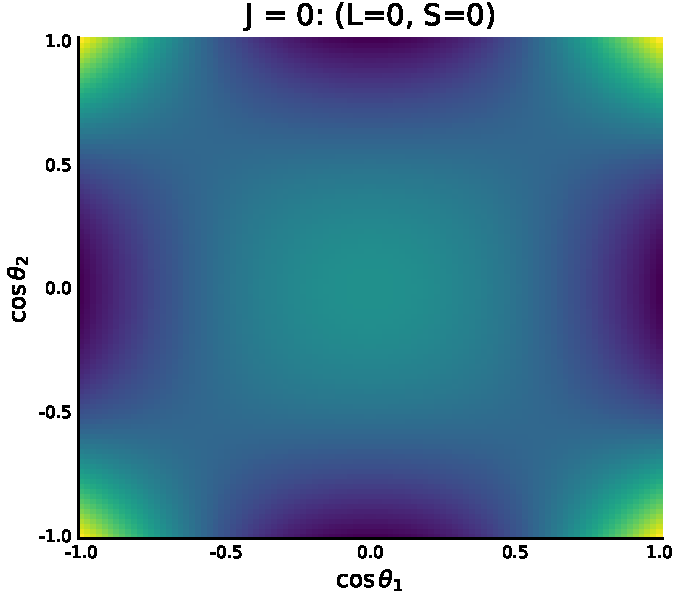
\includegraphics[width=0.195\textwidth]{../plots/map_JLS_000.pdf}
  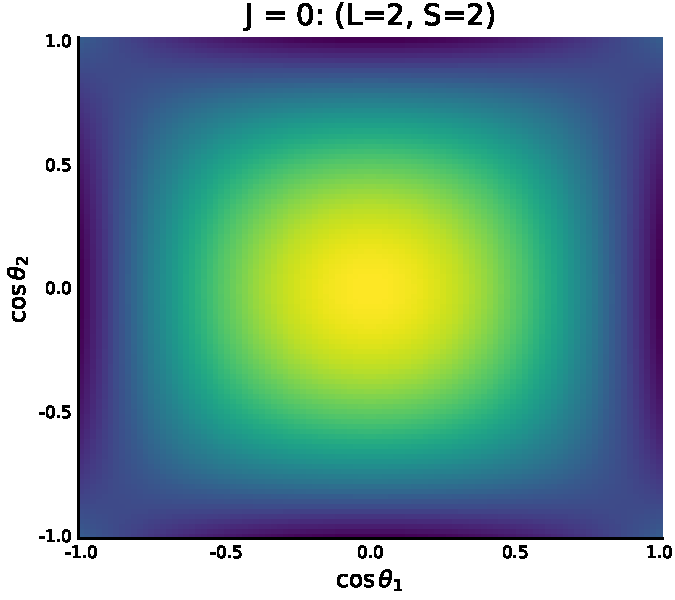
\includegraphics[width=0.195\textwidth]{../plots/map_JLS_022.pdf}
  \caption{}
  \label{fig.j0}
\end{figure}
\begin{figure}
  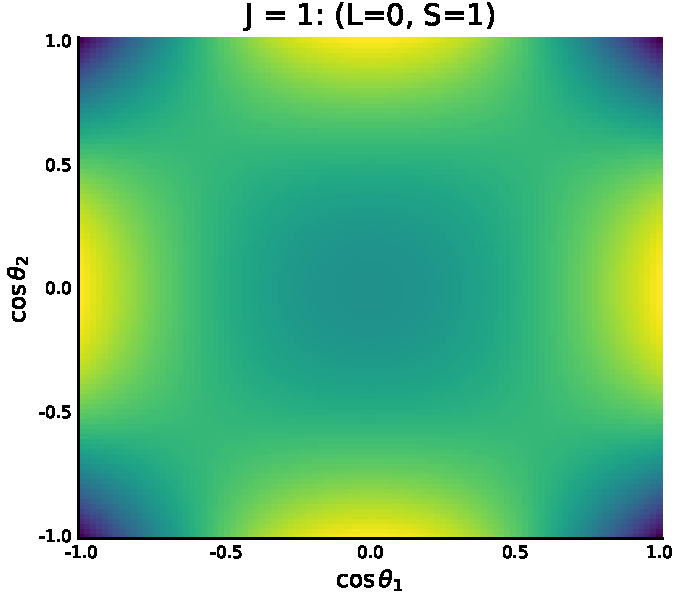
\includegraphics[width=0.195\textwidth]{../plots/map_JLS_101.pdf}
  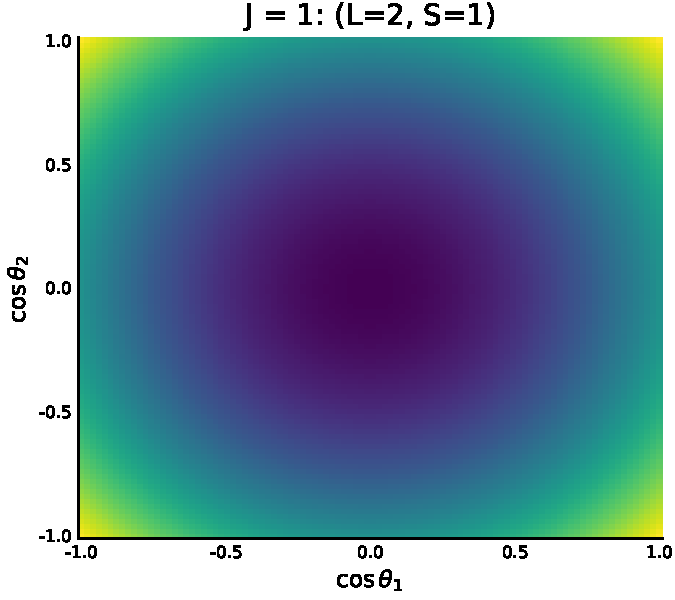
\includegraphics[width=0.195\textwidth]{../plots/map_JLS_121.pdf}
  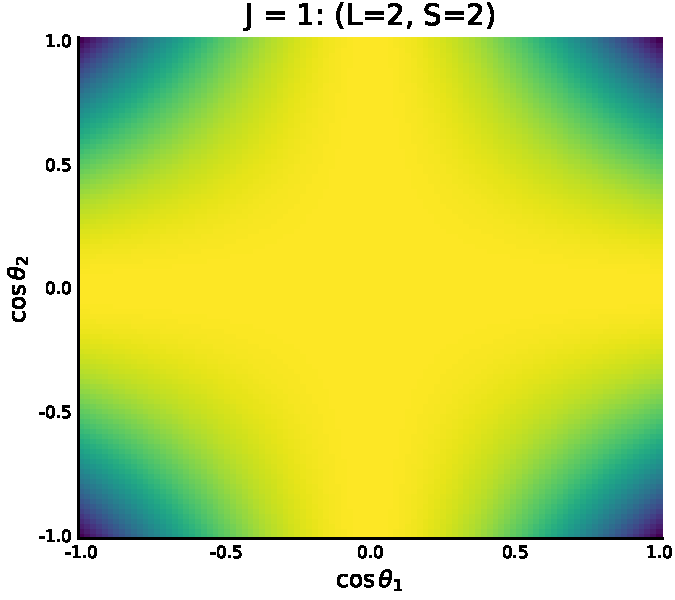
\includegraphics[width=0.195\textwidth]{../plots/map_JLS_122.pdf}
  \caption{}
  \label{fig.j1}
\end{figure}
\begin{figure}
  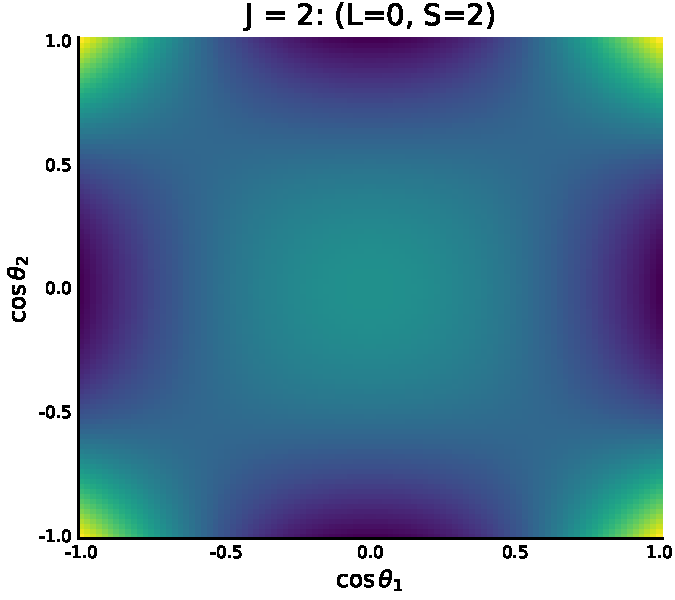
\includegraphics[width=0.195\textwidth]{../plots/map_JLS_202.pdf}
  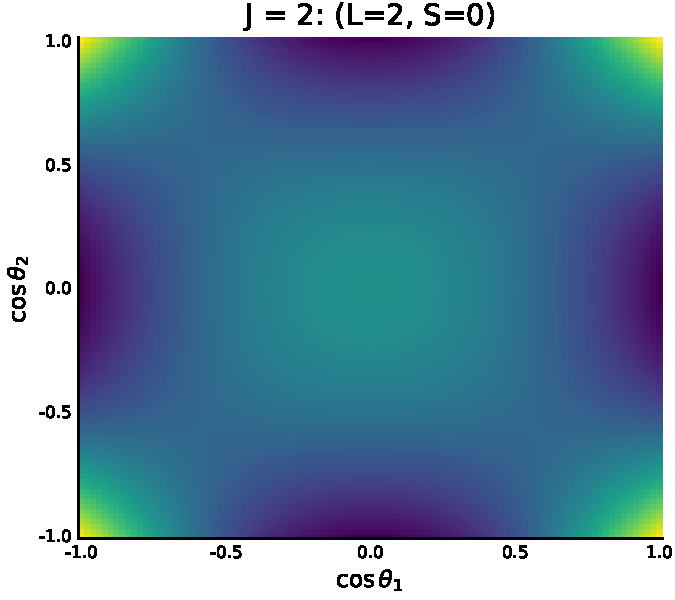
\includegraphics[width=0.195\textwidth]{../plots/map_JLS_220.pdf}
  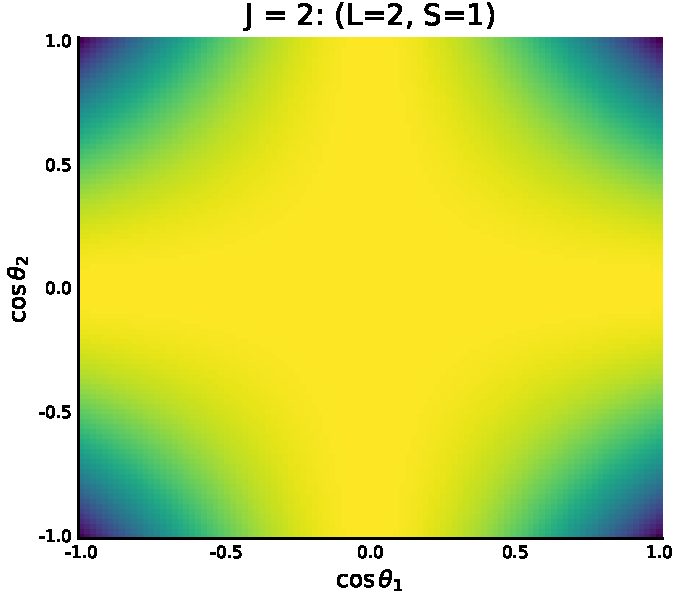
\includegraphics[width=0.195\textwidth]{../plots/map_JLS_221.pdf}
  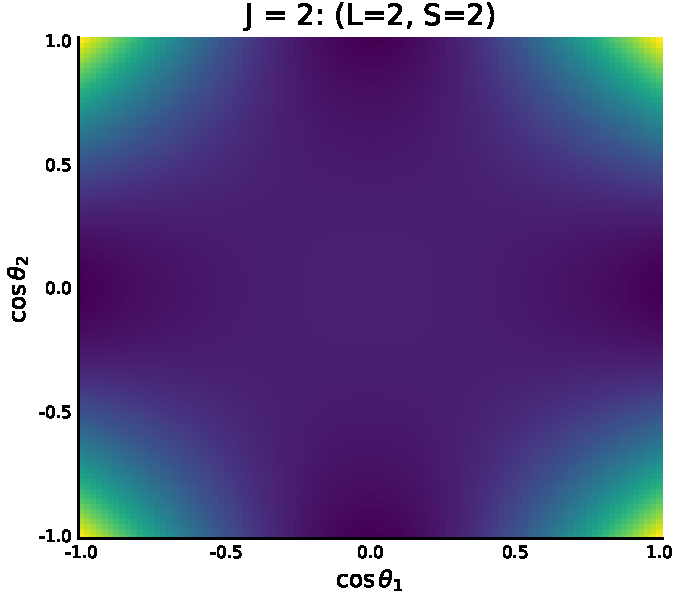
\includegraphics[width=0.195\textwidth]{../plots/map_JLS_222.pdf}
  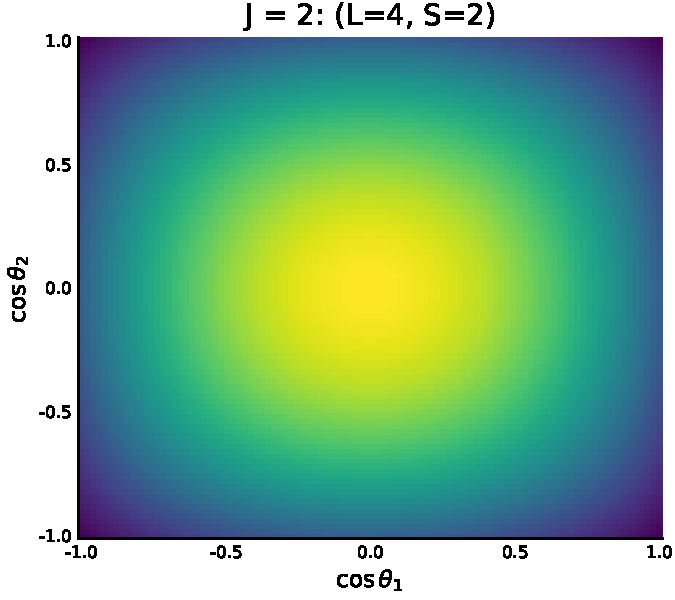
\includegraphics[width=0.195\textwidth]{../plots/map_JLS_242.pdf}
  \caption{}
  \label{fig.j2}
\end{figure}


\bibliography{ref} %%% ref.bib file
\end{document}
